\documentclass[12pt,fleqn]{article}\usepackage{../../common}
\begin{document}
Paralel Rasgele İzdüşümü

Rasgele yansıtma tekniği $m \times b$ boyutunda bir matrisi $n \times k$
boyutunda ve her hücresinde $N(0,1)$ dağılımından gelen bir sayı içeren
matris ile çarpmak sonunda elde edilir. Böylece ana veri matrisi
"yansıtılmış" olur, boyut azaltmak için çok kullanışlı bir tekniktir, çünkü
elde edilen matrisin ana matris $A$'nin "menzilini" iyi temsil ettiği
ispatlanmıştır. Daha fazla detay için bkz [1] yazısı.

Eşle/indirge ortamında rasgele yansıtma için önce [2] adlı yazıya da bakmak
gerekebilir. Bu yazıda iki matris arasındaki çarpıma "satır bakışı" bizim
için gerekli. Çünkü çarpımın solunda $m \times n$ boyutundaki matrisin
verileri bize satır satır geliyor, yani her $m$ satırdan sadece bir
tanesine bakarak işlem yapıyoruz. Faraziyemiz $n$'in de büyük olabilmesine
rağmen en azından $n$ tane veri noktasını tek bir makinada
işleyebileceğimiz.

Satır bakışına dönersek, bu çarpım görüşüne göre soldaki her satır
için, o satırdaki bir öğeyi sağda ona tekabül eden $n \times k$
boyutundaki matrisin satırıyla (yani her gelen satırın 5. öğesi
sağdaki matrisin 5 satırın tamamı ile) çarpıp, sonuç olan "çarpılmış"
satırları birbiriyle topluyoruz. Bu Hadoop veri işleme mentalitesine
uygun çünkü her seferinde $A$'nin tek bir satırına bakıyoruz.

Sağdaki rasgele sayılar içeren matris kritik. Biz bu matrisi bellekte
tut\textbf{ma}maya karar verdik, çünkü $n$ sayısı da büyük olabilir, her
ne kadar $k$ küçük olsa da (çoğunlukla 100 civarı) yine de bu kadar
belleği eğer mümkün ise israf etmemek en iyisi.

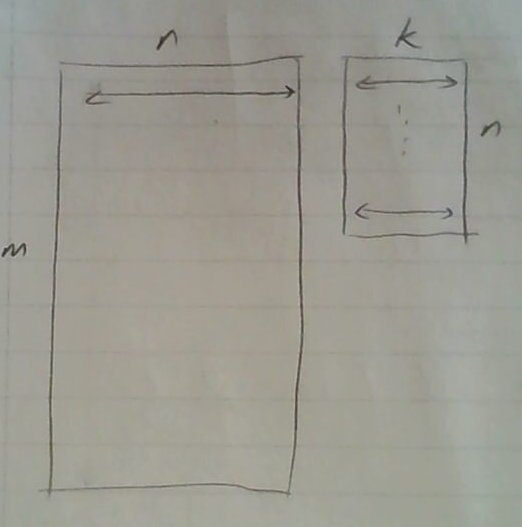
\includegraphics[height=6cm]{proj.png}

Eğer bellekte tutmuyorsak rasgele matrisin değerlerini (sadece
ilgilendiğimiz öğe için, tüm matrisi değil) her seferinde tekrar
üretmek gerekir. Hız açısından performans çok kötü olmayacaktır, çünkü
rasgele sayı üretimi toplama, çarpma, $mod$ gibi direk matematiksel
hesaplar ile yapılır.

Fakat burada önemli bir diğer konu şudur: her $A$ satırı için {\em aynı}
rasgele matris (öğelerini) aynı şekilde üretebilmeliyiz.

Bu problemin en basit çözümü rasgele sayı üretimi için tohum (seed)
kullanımıdır. Eğer tohum kullanılmazsa, Python \verb!random!
paketindeki üretici çağrılar günün zamanına göre bir tohum
kullanırlar, ve böylece her çağrı değişik bir sayı üretmiş olur (çünkü
komut işletildiği her seferinde günün zamanı değişiktir). Fakat
rasgele sayı üretimini, "her seferinde aynı şekilde" yaptırmanın yolku
vardır, bunun için tohum dışarıdan set edilir ve böylece aynı tohumdan
başlayan rasgele sayı üretim zinciri hep aynı olur. Rasgele sayı
üretimi deterministik bir algoritmadır, zaten literatürde bu işlem
"yarı rasgele sayı üretimi (pseudorandom number generation)" olarak
geçer.

\begin{minted}[fontsize=\footnotesize]{python}
import random

# tohumsuz, bu kod her seferinde degisik sayi uretir
print random.gauss(0,1), random.gauss(0,1)
print random.gauss(0,1), random.gauss(0,1)
\end{minted}

\begin{verbatim}
-0.49078710907 1.97156772689
-0.612135407803 -0.0159405924623
\end{verbatim}

\begin{minted}[fontsize=\footnotesize]{python}
import random
# tohumlu
random.seed(100000)
print random.gauss(0,1), random.gauss(0,1)
random.seed(100000)
print random.gauss(0,1), random.gauss(0,1)
\end{minted}

\begin{verbatim}
1.46560757321 0.974749135866
1.46560757321 0.974749135866
\end{verbatim}

Üstteki kodda aynı tohumu verince arka arkaya üretilen iki (daha fazla
da olabilirdi) "rasgele" sayının hep aynı olduğunu görüyoruz.

Rasgele "matrise" dönersek, eğer bu matrisin her $A$ veri satırı için
hücre değerlerinin aynı şekilde üretilmesini istiyorsak, tohum
kullanmalıyız. Tohum değeri ne olacak? Bu değer mesela $n \times k$
boyutundaki rasgele matris için indis değerleri yanyana koyularak
üretilebilir, mesela 111. satır ve 2. kolon için 1112 tohum değeri
kullanılır, ve bu tohumla tek bir rasgele sayı üretilir, (111,2)
hücresine konulur ve sonraki indis için yeni bir tohum
kullanılır. Evet üst üste çakışmalar olabilir tabii ki, mesela
11. satır 12. kolon da üstteki tohumla aynı sonucu getirir, ama bu tür
nadir çakışmalar o kadar önemli değil, sonuçta rasgele sayılarla
uğraşıyoruz, "yeterince raslantısal olmaları" kafi.

Altta bu veri matrisini satır satır çarpıp yansıtılmış yeni bir
matrisi üreten mrjob programını bulabilirsiniz.

\inputminted[fontsize=\footnotesize]{python}{mrproj.py}

Tek bir eşle çağrısı var, çünkü çarpım işlemi oldukça basit, indirgeme
işlemine gerek yok.

Çıktı için yield ile yayınladığımız (emit) satırlarda anahtar
kullanmıyoruz, yani verinin paralel işlenirken nasıl yük dağıtımı
yapıldığına göre sonuç matrisinin sırası ana matrisin satır sırasına
uymayabilir. Fakat satır sırası bizim için çoğunlukla önemli olmuyor
(kolon sırası önemli), çünkü genelde, her satır, diğerinden ayrı /
bağımsız bir veri ölçümünü temsil eder çoğunlukla. Eğer zamansal bir
boyut var ise, bazı şeyler arka arkaya işlenmeliyse, o bilgi ayrı bir
kolon (mesela tarih, zaman damgası -timestamp-) olarak veride
bulunurdu.

\begin{minted}[fontsize=\footnotesize]{python}
!python mrproj.py A_matrix > /tmp/out
\end{minted}

\begin{verbatim}
using configs in /home/burak/.mrjob.conf
creating tmp directory /tmp/mrproj.burak.20131203.094548.254606
writing to /tmp/mrproj.burak.20131203.094548.254606/step-0-mapper_part-00000
Counters from step 1:
  (no counters found)
Moving /tmp/mrproj.burak.20131203.094548.254606/step-0-mapper_part-00000 -> /tmp/mrproj.burak.20131203.094548.254606/output/part-00000
Streaming final output from /tmp/mrproj.burak.20131203.094548.254606/output
removing tmp directory /tmp/mrproj.burak.20131203.094548.254606
\end{verbatim}

\begin{minted}[fontsize=\footnotesize]{python}
!head -10 /tmp/out
\end{minted}

\begin{verbatim}
20.2369671373,13.9358970644,0.524561578258
19.8581349841,13.7724732852,5.23992858318
27.6790861925,18.8833585029,-1.56199395804
9.3255498646,7.52383094482,2.58977793605
27.3677257439,33.0438553532,18.4819155509
27.6790861925,18.8833585029,-1.56199395804
9.3255498646,7.52383094482,2.58977793605
27.3677257439,33.0438553532,18.4819155509
27.6790861925,18.8833585029,-1.56199395804
9.3255498646,7.52383094482,2.58977793605
\end{verbatim}

Performans İyileştirmeleri

Üstteki kod daha hızlı olabilir. Diyelim ki $n$'in milyonlarda olduğu
şartları da hızlı bir şekilde işleyebilmek istiyoruz. Fakat bu noktada
kendimize şu soruyu sormamız gerekir: hangi şartlarda $n$ milyonları
bulacaktır?

Büyük bir ihtimalle bu durum eğer bolca kategorik veri boyutu var ise
ortaya çıkar. Kategorik verileri bildiğimiz gibi 1-in-n, ya da 1-hot
kodlama (encoding) ile temsil ediyoruz, bu demektir ki 1000 tane
farklı değer içerebilen tek bir kolon, 1000 tane yeni kolon haline
geliyor. Bazı boyutların (mesela web sayfa ismi, URL değeri) taşıyan
veri setlerinde özgün (unique) değerlerin milyonlar hatta milyara
varabileceğini düşünürsek aşırı yüksek $n$ rakamlarının nereden
geldiğini anlarız.

Ama bunun bize ek bir faydası var: 1-in-n kodlaması var ise, bu her
satırda çok fazla sıfır olacak demektir, ve içinde çok sıfırı olan
vektörleri / matrisleri seyrek matrisler ile çok rahat şekilde temsil
edebiliriz.

\inputminted[fontsize=\footnotesize]{python}{mrprojs.py}

Üstteki kodda her satırı okur okumaz hemen onu bir seyrek matrise
çeviriyoruz. Şimdi en kritik numara: \verb!itertools.izip!
çağrısı ile bu seyrek matrisin {\em sadece sıfır olmayan değerlerini
ziyaret ediyoruz}. Eğer 1000 tane kolon var ise, ama bu 1000
kolonun 20 tanesi dolu ise, bu 50 kat bir performans iyileştirmesi
sağlayacak demektir (bu arada seyrek verilerde yüzde 2 doluluk gayet
normal bir rakamdır). Sadece dolu hücreleri ziyaret ediyoruz, ayrıca
\verb!izip! bu dolu hücrelerin indis değerlerini de bize geri
getiriyor, biz de bu değerleri \verb!seed! için önceden olduğu
gibi kullanıyoruz. Bir diğer ilerleme $K$ tane rasgele sayıyı bir
kerede üretiyoruz, ve tohum ayarlamasını bir kere, dış döngü başında
gerçekleştiriyoruz. 

Sonuçlara bakalım:

\begin{minted}[fontsize=\footnotesize]{python}
!python mrprojs.py A_matrix > /tmp/out
!head -10 /tmp/out
\end{minted}

\begin{verbatim}
using configs in /home/burak/.mrjob.conf
creating tmp directory /tmp/mrprojs.burak.20131203.094635.908870
writing to /tmp/mrprojs.burak.20131203.094635.908870/step-0-mapper_part-00000
Counters from step 1:
  (no counters found)
Moving /tmp/mrprojs.burak.20131203.094635.908870/step-0-mapper_part-00000 -> /tmp/mrprojs.burak.20131203.094635.908870/output/part-00000
Streaming final output from /tmp/mrprojs.burak.20131203.094635.908870/output
removing tmp directory /tmp/mrprojs.burak.20131203.094635.908870
20.4375200961,1.09117093744,-9.27846872665
13.2830062024,-0.654868464606,-9.66445859893
26.4299520755,0.628144156713,-14.4142094864
9.52053667131,0.337287636006,-3.17826479151
34.6111912648,-0.763663777689,-2.06399979621
26.4299520755,0.628144156713,-14.4142094864
9.52053667131,0.337287636006,-3.17826479151
34.6111912648,-0.763663777689,-2.06399979621
26.4299520755,0.628144156713,-14.4142094864
9.52053667131,0.337287636006,-3.17826479151
\end{verbatim}

Daha önceki sonuçlar ile aynı (rasgelelik var ama \verb!seed!
değerleri değişmedi, o sebeple aynı sonucu aldık, bu iyi).

Bir kontrol daha var, eğer rasgelelik bazlı yansıtma iyi yapıldıysa, $A$
matrisini izdüşümünü aldıktan daha önce anlattığımız teknik ile SVD
hesabını çok rahat bir şekilde yapabilmeliyiz. Bunun için izdüşümünü
\verb!/tmp/Y! içine yazacağız, ve ardından daha önceki QR bazlı
teknikle SVD hesabını yapacağız. Ardından pür SVD ile $A$'yi işleyeceğiz ve
sonuç $U$ matrisindeki en büyük iki eşsiz (singular) değeri her iki
teknikten alıp ekranda grafikleyeceğiz.

\begin{minted}[fontsize=\footnotesize]{python}
!python mrprojs.py A_matrix > /tmp/Y
\end{minted}

\begin{verbatim}
using configs in /home/burak/.mrjob.conf
creating tmp directory /tmp/mrprojs.burak.20140104.064956.493025
writing to /tmp/mrprojs.burak.20140104.064956.493025/step-0-mapper_part-00000
Counters from step 1:
  (no counters found)
Moving /tmp/mrprojs.burak.20140104.064956.493025/step-0-mapper_part-00000 -> /tmp/mrprojs.burak.20140104.064956.493025/output/part-00000
Streaming final output from /tmp/mrprojs.burak.20140104.064956.493025/output
removing tmp directory /tmp/mrprojs.burak.20140104.064956.493025
\end{verbatim}

\begin{minted}[fontsize=\footnotesize]{python}
import numpy.linalg as lin

n = 4; k = 3
A = np.loadtxt('A_matrix')
Y = np.loadtxt("/tmp/Y",delimiter=',')

Q, xx = lin.qr(Y)
B = np.dot(Q.T,A)
Uhat, Sigma, V = lin.svd(B)
U = np.dot(Q, Uhat)

plt.plot(U[:,0],U[:,1],'r+')
plt.hold(True)

U, Sigma, V = lin.svd(A);
plt.plot(U[:,0],U[:,1],'bx')
plt.savefig('rnd_1.png')
\end{minted}

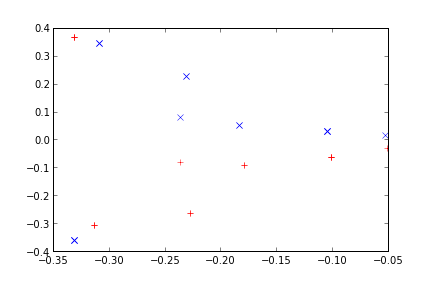
\includegraphics[height=5cm]{rnd_1.png}

Sonuçlar fena değil.

Kaynaklar

[1] Bayramli, Lineer Cebir, {\em Rasgele İzdüşümü ile SVD}

[2] Bayramli, Lineer Cebir, {\em Matris Çarpımı, Ders 1}

\end{document}
